\section{Πιθανοί χειριστές}

Χρήστης/Παίκτης: Ο χειριστής της εφαρμογής απο τον προσωπικό υπολογιστή του. Αλλιώς γνωστός ως "πελάτης".
\newline
Σύστημα/Παιχνίδι: Η εγκατεστημένη εφαρμογή που ανταποκρίνεται στις ενέργειες του χρήστη. Επικοινωνεί με τους διακομιστές. Στο μοντέλο περιπτώσεων χρήσης αντιστοιχίζεται μόνο στα use case που εκτελεί κάτι πέρα απο την εναλλαγή οθονών κλπ. για λόγους ευκρίνειας.
\newline
Βάση Δεδομένων: Η ομάδα σκληρών δίσκων της εφαρμογής που απαρτίζουν τον χώρο αποθήκευσης των δεδομένων των χρηστών. 

\section{Περιπτώσεις χρήσης που θα υλοποιηθούν}
Σε επαρκή λειτουργικότητα θα υλοποιηθούν:
\begin{enumerate}
\item \hyperref[sec:profile]{Εξατομίκευση προγράμματος}
\item \hyperref[sec:buy]{Αγορά αντικειμένου}
\item \hyperref[sec:clanbattle]{Μάχη ομάδας}
\item \hyperref[sec:solo]{Σύστημα μάχης}
\item \hyperref[sec:map]{Χάρτης περιπέτειας}
\item \hyperref[sec:backpack]{Σακίδιο αντικειμένων}
\item \hyperref[sec:createclan]{Δημιουργία ομάδας}
\item \hyperref[sec:friendslist]{Λίστα φίλων}
\end{enumerate}

\newpage
\section{Συνολικό μοντέλο περιπτώσεων χρήσης}

\begin{figure}[htbp]
  
  \centering
    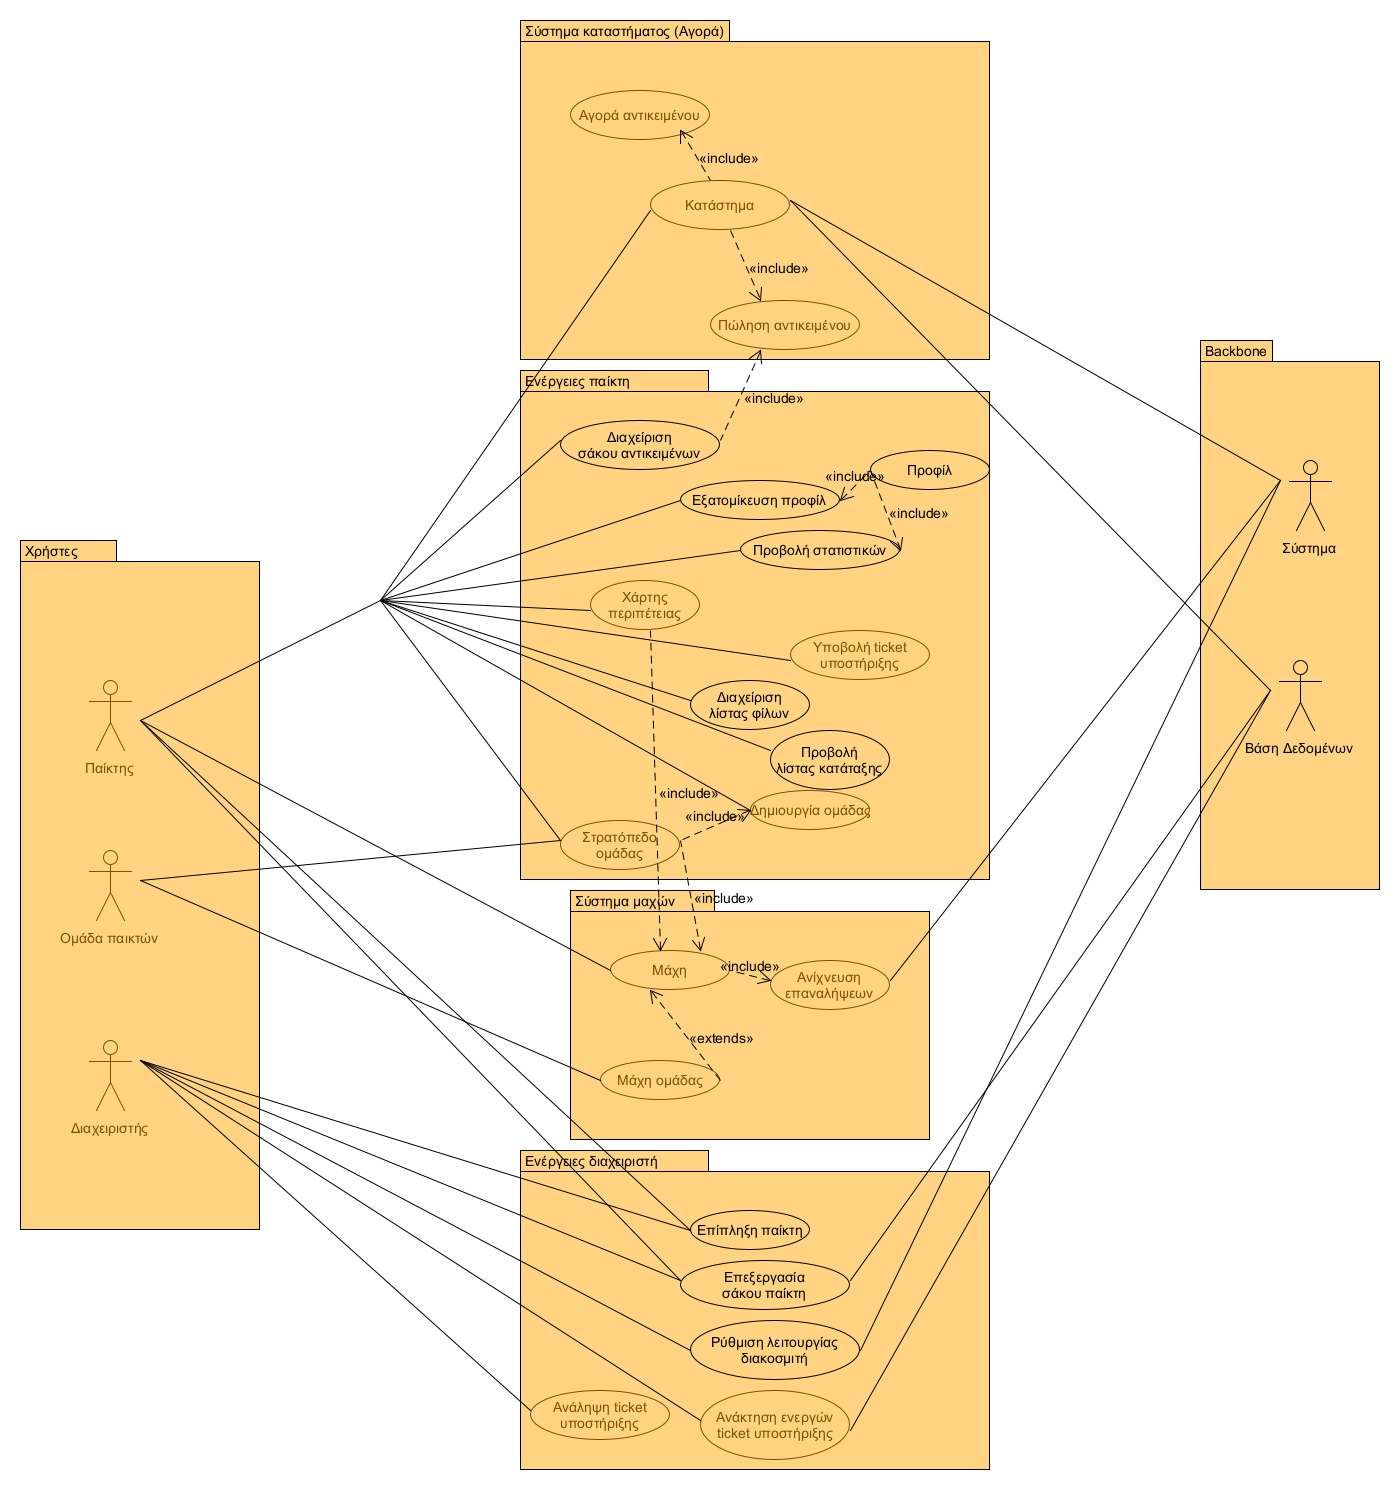
\includegraphics[width=0.9\textwidth]{graphics/uml.png}
    \caption{Rendered using UMLet}
\end{figure}

\newpage
\section{Κείμενα περιπτώσεων χρήσης}
\subsection{Εξατομίκευση προγράμματος}
\label{sec:profile}
\begin{enumerate}
    \item Ο χρήστης επιλέγει μια μάχη.
    \item Το σύστημα ελέγχει εάν ο εγγεγραμμένος χρήστης έχει διαμορφώσει το προφίλ του και διαπιστώνει πως έχει γίνει.
    \item Το σύστημα ανακτά τον ιστορικό μαχών του χρήστη και ελέγχει εάν έχει αθληθεί πολλές φορές σε μικρό χρονικό διάστημα.
    \item Το σύστημα διαπιστώνει πως αυτό δεν έχει γίνει και μέσα από αλγόριθμο προτείνει μερικά προγράμματα γυμναστικής.
    \item Ο χρήστης επιλέγει να ακολουθήσει ένα από αυτά.
    \item Το σύστημα αποθηκεύει την επιλογή του χρήστη και στην μάχη θα εμφανίσει τις ασκήσεις του προγράμματος.
\end{enumerate}

    

Εναλλακτική ροή 1:
\begin{enumerate}[label=3.\alph*.,ref=3.\alph*]
    \item Το σύστημα διαπιστώνει πως αυτό δεν έχει γίνει.
    \item Το σύστημα προωθεί τον χρήστη να διαμορφώσει το προφίλ του.
    \item Ο χρήστης συμπληρώνει διάφορα πεδία και παραμέτρους για να αξιολογηθεί το επίπεδο ενασχόλησης του με την γυμναστική και η φυσική του υγεία.
    \item Το σύστημα ανακτά τις τιμές που εισήγαγε ο χρήστης και μέσα από αλγόριθμο προτείνει μερικά προγράμματα γυμναστικής που δεν έχουν επιλεχθεί ήδη από τον χρήστη.
    \item Ο χρήστης επιλέγει να ακολουθήσει ένα από αυτά.
    \item Το σύστημα αποθηκεύει την επιλογή του χρήστη και στην επόμενη μάχη θα εμφανίσει τις ασκήσεις του προγράμματος.
\end{enumerate}

Εναλλακτική ροή 2:
\begin{enumerate}[label=5.\alph*.,ref=5.\alph*]
    \item Το σύστημα διαπιστώνει πως ο χρήστης έχει αθληθεί πολλές φορές σε μικρό χρονικό διάστημα.
    \item Το σύστημα προτείνει στον χρήστη να ξεκουραστεί, ενημερώνοντάς τον για τους κινδύνους τραυματισμού, ή να κάνει ένα πρόγραμμα γυμναστικής μικρότερης έντασης.
    \item Ο χρήστης επιλέγει αυτό που θέλει, διαβεβαιώνοντας ότι γνωρίζει τους κινδύνους.
\end{enumerate}

Εναλλακτική ροή 3:
\begin{enumerate}[label=6.\alph*.,ref=6.\alph*]
    \item Ο χρήστης επιλέγει να μην ακολουθήσει ένα από αυτά.
    \item Το σύστημα του εμφανίζει τις επιλογές να ακολουθήσει ένα πρόγραμμα που ακολούθησε στο παρελθόν ή να δημιουργήσει δικό του.
    \item Ο χρήστης επιλέγει να δημιουργήσει δικό του πρόγραμμα.
    \item Το σύστημα του εμφανίζει οθόνη με τις ασκήσεις που μπορεί να επιλέξει.
    \item Ο χρήστης επιλέγει τις ασκήσεις και ολοκληρώνει την διαμόρφωση προγράμματός του.
\end{enumerate}



\newpage
\subsection{Αγορά αντικειμένου}
\label{sec:buy}
\begin{enumerate}
    \item Ο χρήστης εισέρχεται στην οθόνη της αγοράς
     \item Το σύστημα εμφανίζει την οθόνη της αγοράς στον χρήστη, με δυνατότητα εφαρμογή φίλτρων.
    \item Το σύστημα ελέγχει εάν υπάρχει σύνδεση με το διαδύκτιο, διαπιστώνει ότι αυτό ισχύει και ανακτά τα πιο δημοφιλή αντικείμενα και τα βάζει πρώτα στην λίστα.
    \item Ο χρήστης εφαρμόζει συγκεκριμένα φίλτρα για να βρει τα αντικείμενα που τον ενδιαφέρουν.
    \item Το σύστημα βρίσκει τα αντικείμενα με βάση την επιλογή φίλτρων και τα εμφανίζει στον χρήστη.
    \item Ο χρήστης επιλέγει το αντικείμενο που θέλει να αγοράσει.
    \item Το σύστημα ελέγχει εάν ο χρήστης έχει αρκετά νομίσματα παιχνιδιού ώστε να αγοράσει το αντικείμενο. Αυτό ισχύει άρα αφαιρεί το ποσό από το υπόλοιπο του χρήστη, επιβεβαιώνει την συναλλαγή και προσθέτει το αντικείμενο στον "σάκο αντικειμένων" του χρήστη.
    \item Το σύστημα επιστρέφει τον χρήστη στην οθόνη της αγοράς.
\end{enumerate}

Εναλλακτική ροή 1:
\begin{enumerate}[label=3.\alph*.,ref=3.\alph*]
    \item Το σύστημα ελέγχει εάν υπάρχει σύνδεση με το διαδίκτυο, διαπιστώνει ότι αυτό δεν ισχύει άρα εμφανίζει κανονικά τα αντικείμενα.
\end{enumerate}

Εναλλακτική ροή 2:
\begin{enumerate}[label=7.\alph*.,ref=7.\alph*]
    \item Το σύστημα διαπιστώνει ένα σφάλμα κατά την επαλήθευση της συναλλαγής. Αναιρεί κάθε προηγούμενη ενέργεια και ενημερώνει τον χρήστη. 
    \item Το σύστημα δίνει στον χρήστη την επιλογή να ξαναπροσπαθήσει την συναλλαγή ή να την ακυρώσει.
    \item Ο χρήστης ξαναπροσπαθεί να αγοράσει το αντικείμενο.
    \item Το σύστημα επαναλαμβάνει τα παραπάνω μέχρι να επαληθευτεί η συναλλαγή.
\end{enumerate}

\newpage
\subsection{Μάχη ομάδας}
\label{sec:clanbattle}
\begin{enumerate}
\item Ο χρήστης επιλέγει να πολεμήσει μαζί με άλλους παίκτες.
\item Το σύστημα ελέγχει εάν ο χρήστης έχει ενεργοποιημένο ίντερνετ και εάν είναι σε κάποια ομάδα. Διαπιστώνοντας πώς ισχύουν και τα δύο του εμφανίζει την επιλογή.
\item Ο χρήστης επιλέγει να προχωρήσει.
\item Το σύστημα ανακτά την πρόοδο της ομάδας και την εμφανίζει στον χρήστη. Εμφανίζει επίσης επιλογές αντιπάλων.
\item Ο χρήστης επιλέγει την μάχη που θέλει να πολεμήσει και ξεκινάει η μάχη ομάδας. Ο τρόπος διεξαγωγής μάχης περιγράφεται στην περίπτωση χρήσης "Σύστημα μάχης".
\item Το σύστημα στέλνει ενημέρωση σε κάθε μέλος της ομάδας.
\item Κάθε χρήστης μέλος της ομάδας μπορεί να πάρει μέρος στην μάχη ομάδας όσες φορές θέλει μέχρι την λήξη του χρονικού ορίου.
\item Κάθε χρήστης μέλος κατά την είσοδό του στη μάχη ομάδας επιλέγει ποιές ασκήσεις (πρόγραμμα γυμναστικής) θα εκτελέσει.
\item Η ομάδα κατατροπώνει τον αντίπαλο στον προαναφερόμενο χρόνο, το σύστημα εμφανίζει κατάλληλο μύνημα σε όλους τους χρήστες μέλη και απονέμει αμοιβές.
\end{enumerate}

Εναλλακτική ροή 1:
\begin{enumerate}[label=2.\alph*.,ref=2.\alph*]
\item Το σύστημα διαπιστώνει πως δεν έχει ενεργοποιημένο ίντερνετ ο χρήστης και σταματάει την είσοδό του. Τον ενημερώνει με κατάλληλο μήνυμα.
\item Ο χρήστης ενεργοποιεί το ίντερνετ.
\item Το σύστημα διαπιστώνει πως πλέον έχει ίντερνετ και συνεχίζει στην επόμενη οθόνη.
\end{enumerate}

Εναλλακτική ροή 2:
\begin{enumerate}[label=2.\alph*.,ref=2.\alph*]
\item Το σύστημα διαπιστώνει πως ο χρήστης δεν ανήκει σε κάποια ομάδα οπότε σταματάει την είσοδό του. Τον ενημερώνει με κατάλληλο μήνυμα. Τον προτρέπει να κάνει εύρεση ομάδας.
\item Ο χρήστης δημιουργεί ή εισέρχεται σε μια ομάδας (περιγράφετια στο use case δημιουργία ομάδας).
\item Το σύστημα ξανακάνει τους ελέγχους και εφόσον διαπιστώσει πως είναι πλέον σε ομάδα εμφανίζει την επόμενη οθόνη.
\end{enumerate}

Εναλλακτική ροή 3:
\begin{enumerate}[label=2.\alph*.,ref=2.\alph*]
\item Η ομάδα δεν προλαβαίνει να κατατροπώσει τον αντίπαλο στον προαναφερόμενο χρόνο.
\item Το σύστημα εμφανίζει μύνημα αποτυχίας σε κάθε χρήστη μέλος.
\end{enumerate}

\newpage
\subsection{Σύστημα μάχης}
\label{sec:solo}
\begin{enumerate}
    \item Ο χρήστης επιλέγει να ξεκινήσει η μάχη.
    \item Το σύστημα, σε συνδυασμό με τις πληροφορίες απο την εξατομίκευση προγράμματος, υπολογίζει τα στατιστικά του αντιπάλου με βάση τo "προφίλ" του χρήστη [σωματική δύναμη, επίπεδό, δύναμη αντικειμένων] και την ζωή που έχει απομείνει στον αντίπαλο απο προηγούμενες μάχες, όλα τα οποία αντλεί απο την βάση δεδομένων.
    \item Το σύστημα εμφανίζει την οθόνη μάχης με τον αντίπαλο, τους πόντους ζωής του και την άσκηση που πρέπει να κάνει ο χρήστης για να πολεμήσει. Σε ένα σημείο της οθόνης εμφανίζει την ζωντανή μετάδοση της κάμερας του χρήστη.
    \item Ο χρήστης πραγματοποιεί επαναλήψεις της άσκησης που του αναγράφεται.
    \item Το σύστημα ανιχνεύει τις επαναλήψεις. Τις αναλύει και ενημερώνει τον χρήστη για την ποιότητα της επανάληψης. Ανανεώνει την οθόνη μειώνοντας τη ζωή του αντιπάλου.
    \item Όταν η ζωή του αντιπάλου φτάσει στο 0, το σύστημα εμφανίζει στον χρήστη το κατάλληλο μύνημα και τις αμοιβές της μάχης [πόντους εμπειρίας, αντικείμενα, νομίσματα].
    \item Ενημερώνει το "προφίλ" του χρήστη στη βάση δεδομένων με τις ανταμοιβές του και καταγράφει το αρχείο της μάχης.
    \item Το σύστημα επιστρέφει τον χρήστη στην οθόνη του χάρτη.
\end{enumerate}

Εναλλακτική ροή 1:
\begin{enumerate}[label=5.\alph*.,ref=5.\alph*]
    \item Περνάει ένα χρονικό διάστημα και το σύστημα δεν εντοπίζει επαναλήψεις.
    \item Το σύστημα εμφανίζει προειδοποιητικό μύνημα στον χρήστη ότι δεν ανιχνέυονται οι επαναλήψεις.
    \item Ο χρήστης διορθώνει την κάμερα και πραγματοποιεί επαναλήψεις.
    \newlineΕναλλακτική Ροή 1.1:
    \begin{enumerate}[label=5.3.\alph*.,ref=5.3.\alph*]
        \item Ο χρήστης δεν αντιδρά -εγκαίρως- στην αίτηση του συστήματος.
        \item Το σύστημα ενημερώνει το χρήστη ότι λόγω αδράνειας ακυρώνεται η μάχη.
        \item Ακολουθείται η εναλλακτική ροή 2.
    \end{enumerate}
    
    \item Το σύστημα εμφανίζει μύνημα επιτυχίας και συνεχίζεται η μάχη.
\end{enumerate}

Εναλλακτική ροή 2:
\begin{enumerate}[label=6.\alph*.,ref=6.\alph*]
    \item Ο χρήστης δεν καταφέρνει να κερδίσει τον αντίπαλο (π.χ. κούραση, ακυρώνει τη μάχη...)
    \item Το σύστημα σταματάει αμέσως την μάχη. Ενημερώνει τον χρήστη ότι δεν θα πάρει ανταμοιβή. Αποθηκεύει την εναπομείναντα ζωή του αντιπάλου.
    \item Ο χρήστης επιστρέφει στην οθόνη του χάρτη.
\end{enumerate}



\newpage
\subsection{Χάρτης περιπέτειας}
\label{sec:map}
\begin{enumerate}
    \item Ο χρήστης εισέρχεται στην οθόνη της περιπέτειας.
    \item Το σύστημα ανακτά την πρόοδο του χρήστη.
    \item Το σύστημα εμφανίζει το χάρτη στο χρήστη και με βάση την πρόοδό που ανέκτησε του δείχνει τα κλειδωμένα επίπεδα, το επίπεδο που μπορεί να επιλέξει και τα ήδη εκπληρωμένα επίπεδα. 
    \item Ο χρήστης επιλέγει επίπεδο.
    \item Το σύστημα φορτώνει την οθόνη μάχης και ζητάει από το χρήστη να στήσει την κάμερά του.
    \item Ο χρήστης στήνει την κάμερά του.
    \item Το σύστημα ανιχνεύει την κάμερα του χρήστη. 
    \item Το σύστημα, χρησιμοποιώντας παραμέτρους του ζωντανού βίντεο, ελέγχει την γωνία της κάμερας και επαληθεύει ότι το μέτρημα των επαναλήψεων μπορεί να γίνει κανονικά.
    \item Το σύστημα φορτώνει την οθόνη μάχης και η μάχη ξεκινάει.
\end{enumerate}


Εναλλακτική ροή 1: 
\begin{enumerate}[label=4.\alph*.,ref=4.\alph*]
\item Ο χρήστης επιλέγει κλειδωμένο επίπεδο.
\item Το σύστημα ενημερώνει το χρήστη πως για να ξεκλειδώσει αυτό το επίπεδο πρέπει πρώτα να ολοκληρώσει τα προηγούμενα.
\item Το σύστημα οδηγεί τον χρήστη στο κομμάτι του χάρτη με το τελευταίο ξεκλειδωμένο επίπεδο.
\item Ο χρήστης επιλέγει ξανά επίπεδο.
\end{enumerate}


Εναλλακτική ροή 2:
\begin{enumerate}[label=6.\alph*.,ref=6.\alph*]
\item Ο χρήστης δεν έχει κάμερα.
\item Το σύστημα δεν ανιχνεύει την κάμερα του χρήστη.
\item Το σύστημα ενημερώνει το χρήστη πως δεν μπορεί να εμπλακεί σε μάχη χωρίς τη χρήση κάμερας.
\item Το σύστημα επιστρέφει το χρήστη πίσω στο χάρτη και δεν το αφήνει να μπει σε μάχη μέχρι να ανιχνεύσει κάμερα.
\end{enumerate}

Εναλλακτική ροή 3:
\begin{enumerate}[label=8.\alph*.,ref=8.\alph*]
\item Το σύστημα δεν μπορεί να εξακριβώσει την οπτική γωνία, με συνέπεια να μην μπορει να εξασφαλίσει σωστό μέτρημα των επαναλήψεων.
\item Το σύστημα ενημερώνει τον χρήστη για αυτό και τον συμβουλεύει να αλλάξει την θέση της κάμερας και να ξαναπροσπαθήσει. 
\item Ο χρήστης συνεχίζει τις αλλαγές μέχρι το σύστημα να μπορεί να εξακριβώσει τα απαραίτητα για την διεξαγωγή της μάχης.
\end{enumerate}

\newpage
\subsection{Σακίδιο αντικειμένων}
\label{sec:backpack}
\begin{enumerate}
\item Ο χρήστης ανοίγει το σακίδιο με τα αντικείμενά του.
\item Το σύστημα φορτώνει μια λίστα με τα αντικείμενα του χρήστη.
\item Ο χρήστης επιλέγει ένα αντικείμενο.
\item Το σύστημα εμφανίζει τις ιδιότητες/χρησιμότητες του αντικειμένου, το κόστος πώλησης και τον αριθμό των αντικειμένων αυτού του τύπου στην κατοχή του χρήστη.
\item Ο χρήστης επιλέγει να χρησιμοποιήσει ένα αντικείμενο.
\item Το σύστημα προσθέτει τις ιδιότητες του αντικειμένου στα στατιστικά του χρήστη και το αφαιρεί από το σακίδιο του χρήστη.
\end{enumerate}

Εναλλακτική ροή 1:
\begin{enumerate}[label=3.\alph*.,ref=3.\alph*]
\item Ο χρήστης επιλέγει ένα αντικείμενο που αποτελεί κομμάτι εξοπλισμού.
\item Το σύστημα δείχνει τα στατιστικά του αντικείμενου και το συγκρίνει με το ήδη φορεμένο κομμάτι εξοπλισμού (αν υπάρχει).
\item O χρήσης επιλέγει να φορέσει το νέο αντικείμενο.
\item Το σύστημα ανανεώνει τα στατιστικά του χρήστη.
\item Το σύστημα αφαιρεί το αντικείμενο από το σακίδιο και προσθέτει στη θέση του το πρώην φορεμένο (αντικατάσταση).
\end{enumerate}

Εναλλακτική ροή 2:
\begin{enumerate}[label=5.\alph*.,ref=5.\alph*]
\item Ο χρήστης επιλέγει να πουλήσει ένα αντικείμενο.
\item Το σύστημα μεταφέρει το χρήστη στην οθόνη της αγοράς.
\item Το σύστημα στέλνει επιβεβαιωτικό μήνυμα για την πώληση του αντικειμένου στο χρήστη.
\item Ο χρήστης επιβεβαιώνει τη συναλλαγή.
\item Το σύστημα προσθέτει τα νομίσματα στο λογαριασμό του χρήστη και αφαιρεί το αντικείμενο από το σακίδιο του χρήστη.
\end{enumerate}

\newpage
\subsection{Δημιουργία ομάδας}
\label{sec:createclan}
\begin{enumerate}
\item Ο χρήστης εισέρχεται στην οθόνη του στρατοπέδου ομάδας.
\item Το σύστημα ενημερώνει τον χρήστη ότι δεν είναι σε ομάδα
\item Το σύστημα προτρέπει τον χρήστη να δημιουργήσει μια δική του ομάδα ή να εισέλθει σε μια ηδη υπάρχων ομάδα.
\item Ο χρήστης επιλέγει να δημιουργήσει μια ομάδα..
\item Μεταβαίνει στην οθόνη δημιουργίας ομάδας.
\item Το σύστημα ζητάει απο τον χρήστη να συμπληρώσει πεδία για τα χαρακτηριστικά της ομάδας και των ρυθμίσεών της.
\item Ο χρήστης δημιουργεί επιτυχώς την ομάδα του.
\item Το σύστημα εμφανίζει την λίστα φίλων του και του προτείνει να προσκαλέσει φίλους του στην ομάδα.
\item Ο χρήστης επιλέγει φίλους του.
\item Το σύστημα αποστέλλει ειδοποίηση στους επιλεγμένους χρήστες φίλους του χρήστη με μια πρόσκληση στην ομάδα.
\item Επιστρέφει στην οθόνη του στρατοπέδου ομάδας.
\end{enumerate}

Εναλλακτική ροή 1:
\begin{enumerate}[label=6.\alph*.,ref=6.\alph*]
\item Διαπιστώνεται ότι μερικά πεδία δεν είναι έγκυρα. Σε περίπτωση στοιχείων όπως όνομα ομάδας, το σύστημα ελέγχει την βάση δεδομένων σε περίπτωση διπλοτυπίας.
\item Η ομάδα δεν δημιουργίεται και επισημαίνονται τα αντίστοιχα πεδία προς διόρθωση. 
\item Ο χρήστης τα διορθώνει και επιβεβαίωνει την δημιουργία ομάδας.
\item Η ομάδα δημιουργείται και η ροή συνεχίζεται κανονικά.
\end{enumerate}

Εναλλακτική ροη 2:
\begin{enumerate}[label=4.\alph*.,ref=4.\alph*]
\item Ο χρήστης επιλέγει να εισέλθει σε μια ήδη υπάρχουσα ομάδα.
\item Το σύστημα εμφανίζει στον χρήστη μια λίστα ομάδων φίλων του.
\item Ο χρήστης επιλέγει μια ομάδα απο τη λίστα.
\item Το σύστημα τον εντάσσει στην ομάδα και αποστέλλει ειδοποίηση στα υπόλοιπα μέλη για την είσοδο του χρήστη.
\item Ο χρήστης μεταβαίνει στην οθόνη του στρατοπέδου ομάδας.
\end{enumerate}

\newpage
\subsection{Στρατόπεδο ομάδας}
\label{sec:clanbase}
\begin{enumerate}
\item Ο χρήστης εισέρχεται στην οθόνη του στρατοπέδου ομάδας.
\item Το σύστημα ανακτά τη λίστα μελών της ομάδας και τα παρουσιάζει στην οθόνη. Φορτώνουν επίσης ενέργειες που μπορεί να κάνει ο χρήστης (συνομιλία ομάδας, μάχη ομάδας, ρυθμίσεις ομάδας, μέλη ομάδας).
\item Ο χρήστης επιλέγει να εμφανίσει τα μέλη της ομάδας.
\item Το σύστημα εμφανίζει τα μέλη της ομάδας με βασικές πληροφορίες τους, με δυνατότητα ενέργειών (όπως στο use case λίστα φίλων).
\item Ο χρήστης επιστρέφει στην προηγούμενη οθόνη.
\end{enumerate}


Εναλλακτική ροή 1:
\begin{enumerate}[label=3.\alph*.,ref=3.\alph*]
\item Ο χρήστης επιλέγει την συνομιλία ομάδας
\item Το σύστημα ανακτά την συνομιλία της ομάδας και την εμφανίζει, με δυνατότητα να γράψει κάτι ο χρήστης.
\item Ο χρήστης αποστέλλει ένα μήνυμα.
\item Το σύστημα προσθέτει στην συνομιλία αυτό το μήνυμα και ενημερώνει τα τους χρήστες μέλη της ομάδας.
\item Ο χρήστης επιστρέφει στην προηγούμενη οθόνη.
\end{enumerate}

Εναλλακτική ροή 2:
\begin{enumerate}[label=3.\alph*.,ref=3.\alph*]
\item Ο χρήστης εισέρχεται στις ρυθμίσεις της ομάδας.
\item Εμφανίζεται η οθόνη ρυθμίσεων και διάφορα χαρακτηριστικά της ομάδας (όνομα, επιλογή διαγραφής, αρχηγός ομάδας, ...).
\item Ο χρήστης τροποποιεί κάποιο πεδίο.
\item Το σύστημα ζητάει επιβεβαίωσει. Στη συνέχεια, εφαρμόζει την αλλαγή και ενημερώνονται τα στοιχεία της ομάδας.
\end{enumerate}

Εναλλακτική ροή 2.2:
\begin{enumerate}[label=3.3.\alph*.,ref=3.3.\alph*]
\item Ο χρήστης δεν έχει τα κατάλληλα δικαιώματα ώστε να τροποποιήσει τις ρυθμίσεις τις ομάδας.
\item Το σύστημα εμφανίζει τα αντίστοιχα πεδία ως μη τροποποιήσιμα.
\item Ο χρήστης προσπαθεί να τροποποιήσει κάποιο πεδίο.
\item Το σύστημα τον ενημερώνει πως δεν έχει τα κατάλληλα δικαιώματα για αυτή την κίνηση.
\end{enumerate}




\newpage
\subsection{Λίστα φίλων}
\label{sec:friendslist}
\begin{enumerate}
\item Ο χρήστης απο την κύρια οθόνη εισέρχεται στην οθόνη της λίστας φίλων.
\item Το σύστημα ελέγχει εάν υπάρχει σύνδεση στο διαδίκτυο.
\item Το σύστημα διαπιστώνει πως αυτό ισχύει και ανακτά τους φίλους του χρήστη και τους εμφανίζει, με δυνατότητα διαγραφής και προσθήκης νέου φίλου και πρόσκλησης στην ομάδα του χρήστη.
\item Ο χρήστης επιλέγει την προσθήκη νέου φίλου εισάγοντας το όνομα του παίκτη που θέλει να προσθέσει.
\item Το σύστημα ελέγχει το όνομα ώστε να υπάρχει στην βάση δεδομένων και επιστρέφει ενημερωτικό μήνυμα. Στέλνει αίτημα στον άλλο παίκτη.
\item Ο χρήστης εξέρχεται από τα μενού προσθήκης φίλου.
\item Το σύστημα εμφανίζει επιλέον ενημερωτικό μήνυμα εάν ο άλλος παίκτης δεχθεί το αίτημα.
\end{enumerate}

Εναλλακτική Ροή 1:
\begin{enumerate}[label=3.\alph*.,ref=3.\alph*]
\item Το σύστημα βλέπει πως η συσκευή δεν έχει πρόσβαση στο διαδίκτυο.
\item Το σύστημα ανακτά την πιο πρόσφατα cached λίστα φίλων και την εμφανίζει.
\item Ο χρήστης δεν μπορεί να εκτελέσει περαιτέρω ενέργειες, αφού είναι σε view-only ενός αντίγραφου της λίστας φίλων.
\end{enumerate}

Εναλλακτική Ροή 2:
\begin{enumerate}[label=4.\alph*.,ref=4.\alph*]
\item Ο χρήστης επιλέγει να λάβει υπερσύνδεσμο για το αίτημα φιλίας.
\item Το σύστημα εφόσον είναι συνδεδεμένο στο διαδίκτυο παράγει και εμφανίζει τον υπερσύνδεσμο που αρμόζει στον χρήστη.
\item Η ροή συνεχίζεται απο το βήμα 6 της κανονικής ροής.
\end{enumerate}

Εναλλακτική Ροή 3:
\begin{enumerate}[label=5.\alph*.,ref=5.\alph*]
\item Το σύστημα βρίσκει πως ο παίκτης με το εισαχθέντο όνομα δεν υπάρχει στην Β.Δ.
\item Ο χρήστης επαναλαμβάνει την εισαγωγή ονόματος, επανέρχοντας στην κανονική ροή στο βήμα 4.
\end{enumerate}

Εναλλακτική ροή 4:
\begin{enumerate}[label=4.\alph*.,ref=4.\alph*]
\item Ο χρήστης επιλέγει να διαγράψει έναν φίλο του.
\item Το σύστημα ανανεώνει την βάση δεδομένων και τον επιστρέφει στην λίστα φίλων.
\end{enumerate}

Εναλλακτική ροή 5:
\begin{enumerate}[label=4.\alph*.,ref=4.\alph*]
\item Ο χρήστης επιλέγει να προσκαλέσει έναν φίλο του στην ομάδα του.
\item Το σύστημα στέλνει αίτημα στον άλλο παίκτη και τον επιστρέφει στην λίστα φίλων.
\end{enumerate}

\newpage
\section{Λοιπές περιπτώσεις χρήσης}
Εδώ αναγράφονται οι περιπτώσεις χρήσεις που δεν έχουν βασική και εναλλακτική ροή. Παρατίθενται μόνο για την πληρότητα του τεχνικού κειμένου.
\subsection{Προβολή στατιστικών}
\subsection{Πώληση αντικειμένου}
\subsection{Υποβολή ticket υποστήριξης}
\subsection{Ανίχνευση επαναλήψεων}
\subsection{Επίπληξη παίκτη}
\subsection{Επεξεργασία σάκου παίκτη}
\subsection{Ανάληψη ticket υποστήριξης}
\subsection{Ανάκτηση ενεργών ticket υποστήριξης}
\subsection{Ρύθμιση λειτουργίας διακοσμιτή}